\documentclass[10pt,a4paper]{article}

\usepackage[margin=1in]{geometry}
\usepackage[UKenglish]{babel}
\usepackage{enumitem}
\usepackage{calc}
\usepackage{fancyhdr}
\usepackage{graphicx}
\usepackage{multirow}
\usepackage[table]{xcolor}
\usepackage{float}
\usepackage{longtable}
\usepackage{parskip}
\usepackage{soul}
\usepackage{ifthen}
\usepackage[compact]{titlesec}
\usepackage[justification=centering]{caption}
\usepackage{subcaption}
\usepackage{listings}
\usepackage{xcolor}

\colorlet{punct}{red!60!black}
\definecolor{background}{HTML}{EEEEEE}
\definecolor{delim}{RGB}{20,105,176}
\definecolor{key}{RGB}{73,109,112}
\colorlet{numb}{magenta!60!black}

\lstdefinelanguage{json}{
    basicstyle=\normalfont\ttfamily,
    numbers=left,
    numberstyle=\scriptsize,
    stepnumber=1,
    numbersep=8pt,
    showstringspaces=false,
    breaklines=true,
    frame=lines,
    backgroundcolor=\color{background},
    literate=
     *{0}{{{\color{numb}0}}}{1}
      {1}{{{\color{numb}1}}}{1}
      {2}{{{\color{numb}2}}}{1}
      {3}{{{\color{numb}3}}}{1}
      {4}{{{\color{numb}4}}}{1}
      {5}{{{\color{numb}5}}}{1}
      {6}{{{\color{numb}6}}}{1}
      {7}{{{\color{numb}7}}}{1}
      {8}{{{\color{numb}8}}}{1}
      {9}{{{\color{numb}9}}}{1}
      {:}{{{\color{punct}{:}}}}{1}
      {,}{{{\color{punct}{,}}}}{1}
      {\{}{{{\color{delim}{\{}}}}{1}
      {\}}{{{\color{delim}{\}}}}}{1}
      {[}{{{\color{delim}{[}}}}{1}
      {]}{{{\color{delim}{]}}}}{1},
}
\lstset{emph={%  
    Systems, SystemID, Sensors, SensorID, Params, Engines, DatastoreGateway, Reporting
    },emphstyle={\color{key}\bfseries}%
}

\definecolor{reqColor}{RGB}{80,80,120}

%%Tables
\newcommand{\tableformat}[4]{
\begin{table}[t]
\centering
  \rowcolors{2}{gray!10} {white}
\begin{tabular}{#1}
  \hline
  \rowcolor[gray]{0.9} #2
\end{tabular}
\caption{#3}
\label{#4}
\end{table}}

\pagestyle{fancy}
\lhead{T Davies, A Fahie, A Fairbairn, A Free, J Mansfield, R Tucker, M 
Walker}
\chead{}
\rhead{GPIG-C}
\cfoot{\vspace{-0.6cm} \thepage}

\setlist{nolistsep} % Reduces lots of white space around lists

\renewcommand{\headrulewidth}{0.4pt} % Add rules below header
\renewcommand*{\thefootnote}{\fnsymbol{footnote}}

\newcommand{\conreq}[1]{\textcolor{reqColor}{\textbf{CR.#1}}}
\newcommand{\fr}[1]{\textcolor{reqColor}{\textbf{FR.#1}}}
\newcommand{\ed}[1]{\textcolor{reqColor}{\textbf{ED.#1}}}
\newcommand{\nfr}[1]{\textcolor{reqColor}{\textbf{NFR.#1}}}
\newcommand{\qas}[1]{\textcolor{reqColor}{\textbf{QAS.#1}}}
		
		


%%Scenarios
\newenvironment{scenario}[1]{
\newcommand{\source}[1]{\item[Source of Stimulus:] ##1}
\newcommand{\stimulus}[1]{\item[Stimulus:] ##1}
\newcommand{\artifact}[1]{\item[Artifact:] ##1}
\newcommand{\environment}[1]{\item[Environment:] ##1}
\newcommand{\response}[1]{\item[Response:] ##1}
\newcommand{\measure}[1]{\item[Response Measure:] ##1}
\newcommand{\rationale}[1]{\item[Scenario Rationale:] ##1}
\newcommand{\quality}[1]{\item[Quality:] ##1}
		\begin{description} [noitemsep]	
		\item[Scenario ID:] \qas{#1}
		}{\end{description} \vspace*{0.3cm}
		}

%%Requirements
\newenvironment{requirements}{
\newcommand{\requirement}[4]{\item[##1{##2}] ##3
							\ifx&##4&
							%nothing
							\else
								\begin{description}
									##4
								\end{description}							
							\fi
							}
		\begin{description}[noitemsep, leftmargin=1.3cm]	
		}{\end{description} \vspace*{0.3cm}
		}
		
\begin{document}
\begin{center}
{\vspace*{-0.5cm}
\Huge GPIG-C Final Report}
\vspace*{0.2cm}

Word count: % @WORD_COUNT@
 (\textit{using TeXCount})
\vspace*{0.1cm}

Wednesday, 21st May 2014
\end{center}
\vspace*{0.4cm}
\hrule
\vspace*{0.4cm}

%-------------------------------------------------------------%
%----------------------INTRODUCTION -------------------%
%-------------------------------------------------------------%
\section{Introduction}
\label{sec:intro}
This report details the design and development of our HUMS, concentrating on progress made since the interim report. System requirements are further refined, building on feedback from previous reports, adding a set of external dependencies. The HUMS architecture is then considered, in order to determine how the System will meet its requirements and what design decisions must be made. This includes examining the important quality attributes of the system and related scenarios, as well as the tactics and patterns which can be used to achieve these qualities. Our desired HUMS architecture is then presented using a number of views, deemed to be important. Having determined the HUMS architecture, the associated risks with the project as a whole are considered, and risk reduction tactics are discussed.

The development of the prototype HUMS, demonstrating some of the important features in the design, is then described, followed by a set of evaluations used to determine the achieved quality and functionality of the System. The project is then concluded, and the team reflects on their decisions throughout the project.

%-------------------------------------------------------------%
%--------------------------GLOSSARY ---------------------%
%-------------------------------------------------------------%
\section{Glossary}
\label{sec:glossary}
\hl{TODO: Tom}
\begin{description}%[leftmargin=!,labelwidth=\widthof{\bfseries Data output clientxx},noitemsep]
	\item[The HUMS/System] The health and usage monitoring system being developed
	\vspace{0.15cm}
	\item[Customer] Thales, the organisation that has commissioned the System
	\item[Consumer] An organisation that makes use of the System
	\item[Consumer System] The system that a Consumer wishes to monitor
	\item[(End) User] An individual that uses the System within a Consumer organisation
	\vspace{0.15cm}
	\item[Client] Computer hardware or software that interfaces with an Instance
	\item[Input Interface] The interface through which data is supplied to an Instance
	\item[Data Emitter] A Client that provides data to an Instance through the Input Interface
	\item[Output Interface] The interfaces through which reports and notifications are dispatched
	\item[Data Output Client] A Client that receives data from an Instance through Output Interfaces
    \item[Data Store] The component of the System which stores data received through the Input Interface.
	\item[Admin Centre] Web interface to configure and interact with the Core.
	\item[(HUMS) Core] The component of the System which performs analysis, and which receives data from Data Emitters through the Input Interface.
	\vspace{0.15cm}
	\item[Event] A trend in data identified by analysis
	\item[Notification] A message dispatched by the System when an Event is fired
	\item[Report] A message produced by the System at the request of a User
	\vspace{0.14cm}
	\item[Sensor] A source of data to be monitored by the System
	\item[Sensor ID] A unique identifier denoting a particular Sensor
	\item[System ID] A unique identifier denoting a group of Sensors
\end{description}

%-------------------------------------------------------------%
%-------------------REQUIREMENTS----------------------%
%-------------------------------------------------------------%
\section{Requirements Refinement}
\label{sec:requirements}
After feedback from the initial and interim reports, the HUMS requirements have been updated. This included modifying existing requirements and adding additional requirements and refinements. It also included removing the constraint requirements, which were deemed unnecessary by the module leader, and instead identifying the external dependencies of the system.

\subsection{Functional Requirements}
\label{sec:functional_requirements}

\emph{FR.4.1.1} and \emph{FR.4.1.2} were added as we implemented configuration files into our prototype. We chose to use \emph{JSON} as the configuration format as it is a widely-used standard.

\emph{FR.12} became apparent once we considered the reloading of configuration in \emph{FR.4.1.2}, as without the ability to load new engines, adding new analyses and reporting methods would require a restart of the System to take effect.

\begin{requirements}
\requirement{\fr}{1}{Data Emitters shall be able to push correctly structured data to the HUMS.}{
	\requirement{\fr}{1.1}{The HUMS shall provide an API for data input (the Input Interface).}{
		\requirement{\fr}{1.1.1}{The Input Interface shall require a System ID that uniquely identifies the Consumer System.}{}
		\requirement{\fr}{1.1.2}{The Input Interface shall require input data to be timestamped.}{}
		\requirement{\fr}{1.1.3}{The Input Interface shall allow Data Emitters to send Sensor IDs and their values to the HUMS, to be made available to an analysis engine.}{}
	}
	\requirement{\fr}{1.2}{A Data Emitter for extracting data from the given test application shall be provided.}{}
}
\requirement{\fr}{2}{The HUMS shall allocate a timestamp to new data.}{
	\requirement{\fr}{2.1}{Data shall be timestamped before it reaches the HUMS Input Interface.}{}
	\requirement{\fr}{2.2}{Timestamps shall be stored alongside the input data.}{}
}
\requirement{\fr}{3}{The HUMS shall store correctly structured data.}{
	\requirement{\fr}{3.1}{The HUMS shall use a database abstraction layer, allowing the Consumer to select their datastore technology.}{}
}
\requirement{\fr}{4}{The HUMS shall store Consumer configuration files.}{
	\requirement{\fr}{4.1}{The HUMS shall allow authorised Users to modify configuration files.}{
      \requirement{\fr}{4.1.1}{The Admin Centre shall provide an interface to allow authorised users to modify the configuration.}{}
      \requirement{\fr}{4.1.2}{The HUMS shall monitor the configuration for changes and apply them.}{}
    }
	\requirement{\fr}{4.2}{The HUMS shall allow the User to define a storage limit.}{}
	\requirement{\fr}{4.3}{The HUMS shall allow the User to set an expiry time on stored data.}{}
	\requirement{\fr}{4.4}{The HUMS shall allow the User to define that, upon reaching their defined data storage quota, new data is no longer stored.}{}
	\requirement{\fr}{4.5}{The HUMS shall allow the User to define that, upon reaching their defined data storage limit, old data is removed to make room for the new data.}{}
}
\requirement{\fr}{5}{The HUMS shall dispatch a Notification when the Consumer's storage limit is reached.}{}
\requirement{\fr}{6}{The HUMS shall store no more data records than the Consumer-defined storage quota.}{}
\requirement{\fr}{7}{Events shall be triggered in response to data matching analysis rules specified by a User.}{
	\requirement{\fr}{7.1}{The HUMS shall allow the User to specify which analysis rules will produce Events.}{}
	\requirement{\fr}{7.2}{The HUMS shall allow the User to define their own Events.}{}
	\requirement{\fr}{7.3}{The HUMS shall provide an API, allowing analysis engines to fetch stored data.}{}
	\requirement{\fr}{7.4}{Events shall be identified by analysis engines.}{}
	\requirement{\fr}{7.5}{The HUMS shall provide a simple analysis engine in the form of a rules engine.}{}
}
\requirement{\fr}{8}{After dispatching a Notification for an Event of a particular type, no more Notifications for an Event of that type will be sent during a User-specified cool down period.}{
	\requirement{\fr}{8.1}{The HUMS shall allow the User to specify a cool down period for particular Events.}{}
}
\requirement{\fr}{9}{The HUMS shall identify an Event when a specified analysis rule is matched.}{}
\requirement{\fr}{10}{The HUMS shall interface with Report engines, allowing them to pull Reports.}{}
\requirement{\fr}{11}{The System shall allow for Notifications to be fed back to the Consumer System to change
the way in which data is sensed.}{}
\requirement{\fr}{12}{The System shall load new engines which an authorised user adds during runtime.}{}
\end{requirements}

\subsection{Non-Functional Requirements}
\label{sec:nonfunctional_requirements}
\hl{more changes?} 

\emph{NFR.14} was added as it is not necessarily the case that an Consumer will want to use the Admin Centre to modify the configuration file, in which case it should be possible to manually amend the file.

\begin{requirements}
\requirement{\nfr}{1}{The HUMS shall undergo hardware modifications without loss of previously stored data.}{}
\requirement{\nfr}{2}{Users shall be provided with documentation detailing how to use the HUMS.}{}
\requirement{\nfr}{3}{The HUMS shall be accessible to Consumers regardless of their geographic location.}{}
\requirement{\nfr}{4}{The HUMS shall only accept data from a Client of the Input Interface providing valid credentials.}{}
\requirement{\nfr}{5}{The HUMS shall allow data to be stored according to the relevant industry security standards.}{}
\requirement{\nfr}{6}{The HUMS shall be tested to ensure all requirements are met before deployment.}{
	\requirement{\nfr}{6.1}{The HUMS shall be tested using unit testing.}{}
	\requirement{\nfr}{6.2}{The HUMS shall be tested using integration testing.}{}
	\requirement{\nfr}{6.3}{The HUMS shall be tested using system testing.}{}
	\requirement{\nfr}{6.4}{The HUMS shall be tested using inspection.}{}
	\requirement{\nfr}{6.5}{The HUMS shall be tested using acceptance testing.}{}
}
\requirement{\nfr}{7}{The Customer will complete acceptance testing before the System is deployed.}{}
\requirement{\nfr}{8}{The System shall be able to support at least 5 Clients of the Output Interface per HUMS Instance.}{}
\requirement{\nfr}{9}{The System shall be available for no less than 99.9\% of each month.}{}
\requirement{\nfr}{10}{Data shall be backed up within 24 hours of having been made available to the System.}{}
\requirement{\nfr}{11}{Timestamps applied by the system shall be accurate to within 5 ms of UTC.}{}
\requirement{\nfr}{12}{The System shall dispatch Notifications within 5 ms of an Event being triggered.}{}
\requirement{\nfr}{13}{The System shall support storing data without requiring specific schemata.}{}
\requirement{\nfr}{14}{The configuration shall be in a human-readable format.}{}
\end{requirements}

\subsection{External Dependencies}
 \label{sec:external_dependencies}
\hl{todo --- write an intro to these, 4 dependencies is probably enough}

 \begin{description}
 \item[\ed{1}] \hl{todo}
 \item[\ed{2}] \hl{todo}
 \item[\ed{3}] \hl{todo}
 \item[\ed{4}] \hl{todo}
 \end{description}


%-------------------------------------------------------------%
%-----------------------QUALITIES-------------------------%
%-------------------------------------------------------------%
\section{Quality Attributes}
\label{sec:qualities}
A number of quality attributes must be considered when creating the HUMS architecture in order to ensure that architectural decisions not only provide the desired functionality but produce a system meeting the needs of all stakeholders.
Defining these attributes explicitly allows tactics and patterns to be adopted at an early stage, allowing the system to achieve the desired utilities of each quality. 
When considering the HUMS, its requirements and its stakeholders, Table~\ref{tab:qualities} ranks the qualities associated with the system, and explains why each quality was given a particular ranking. The ranking of qualities was not done in the previous report, however is important as optimising the utility of one attribute may result in the utility of another being reduced. Achieving the right balance is therefore very important, and the utility of lower ranked qualities may need to be sacrificed in order to obtain the required utility of highly ranked qualities. Tailorability is important to the Customer, and has been decomposed into a number of sub qualities: Modifiability, Configurability, and Interoperability.

\tableformat{p{2.4cm} p{1.2cm} p{11.2cm}}{
\hline
Quality \qquad Attribute & Rank & Reasoning \\
\hline
Configurability & High & It is important that the HUMS can be used in a range of domains; this has been strongly emphasised by the customer. 
\\
Modifiability & High & The HUMS will initially be built to tackle a single domain (software applications), however, in the future it will be used in domains such as embedded, electrical, and mechanical systems. A system which is not modifiable will be timely and costly to extend. In addition, both users and developers need to be able to add custom engines to the HUMS.
\\
Interoperability & High & Interoperability is very important to the HUMS as its main purpose is to interface and exchange data with external systems. 
\\
Availability & High & The non-functional system requirements identified high availability targets for the system. In addition, the HUMS is designed to be used to monitor the health of other systems so if it was not highly available then Consumers would lose confidence in it. The HUMS must be at least as available as the average Consumer's system in order to monitor it properly. 
\\
Security & High & Security is highly ranked as data being monitored must be kept both confidential and safe. It must be impossible for an unauthorised user to view or modify system data, and data in transit between Data Emitters and the HUMS must be protected.
\\
Performance & Medium & The HUMS is required to receive data from Sensors, and produce Notification events in response to that data with a latency no greater than 5 ms. It must also interface with many Data Emitters and Data Output Clients, meaning it must be capable of handling a large number of events quickly.
\\
Testability & Medium & The TDD development approach, discussed in the initial report and followed throughout the project, makes testability of medium importance to the system. Having a high testability utility will help to reduce system faults and is also likely to increase its availability. 
\\
Usability & Low & Usability was not deemed of great importance to the system as its sub-qualities, such as helpfulness and learnability, have little scope to be optimised in the HUMS. Usability does need to be considered for the web interface and admin centre, however this is only a small part of the HUMS.
\\
}{The ranked quality attributes, associated with the HUMS}{tab:qualities}

%-------------------------------------------------------------%
%----------------------SCENARIOS---------------------%
%-------------------------------------------------------------%
\section{Quality Attribute Scenarios}
\label{sec:scenarios}
Having identified the quality attributes which are important to creating a successful system, a set of quality attribute scenarios can be created which show how the system should respond to certain stimuli. This helps to create goals which the final implementation can be tested against to determine its quality and how effective it is at achieving its non-functional requirements. The selection of scenarios presented below are included as they appear particularly interesting and describe how the system should behave both normally and in extreme conditions. Other scenarios where also considered and documented, however could not be included in this report due to space limitations.

\begin{scenario}{1}
\quality{Configurability}
\source{The Customer}
\stimulus{The Customer wishes to reconfigure the system to monitor mechanical systems.}
\artifact{HUMS Core}
\environment{Design Time}
\response{The System is reconfigured to be comparable with mechanical systems, tested, and deployed.}
\measure{All work is completed on time and in budget.}
\rationale{This scenario is important to the customer, as they expect the HUMS to move across domains easily.}
\end{scenario}

\begin{scenario}{2}
\quality{Modifiability}
\source{Developer}
\stimulus{The Customer wishes to add an additional analysis, reporting, or notification engine to the HUMS.}
\artifact{HUMS Core}
\environment{Runtime}
\response{The new engine is implemented, tested and successfully added to the HUMS, without any loss in service.}
\measure{No other system elements are affected, and the work is completed within budget.}
\rationale{This scenario is important to both the HUMS developers and the Consumers. The HUMS should allow both of these groups to add custom engines to the system without affecting other system components.}
\end{scenario}

\begin{scenario}{3}
\quality{Security}
\source{An unknown external Client}
\stimulus{The unknown external Client attempts to access stored HUMS data or HUMS services.}
\artifact{HUMS Core}
\environment{Normal Operation -- Online}
\response{The Client is authenticated, and allowed to access system services, or is not recognised and blocked from accessing system data and services.}
\measure{No HUMS data or services are damaged as a result of the access attempt.}
\rationale{This scenario shows how the HUMS is expected to behave when a Client attempts access to its services, showing the importance of authenticating Clients and how the HUMS should respond to unauthorised Clients.}
\end{scenario}

\begin{scenario}{4}
\quality{Availability}
\source{Datastore Module}
\stimulus{The Consumer's registered datastore is unavailable to the HUMS instance.}
\artifact{HUMS}
\environment{Runtime}
\response{A Notification is sent to the administrator of the HUMS instance, and the HUMS periodically attempts to reconnect to the Datastore.}
\measure{End user defined repair time.}
\rationale{This scenario shows how the HUMS should respond to a datastore failure, clearly drawing a line between the responsibilities of the HUMS and of the Consumer. If the Consumer's defined datastore fails the HUMS can only alert the user and attempt to reconnect -- this is a critical fault and does not allow the system to be run in a degraded mode.}
\end{scenario}

%-------------------------------------------------------------%
%--------------------------RISKS--------------------------%
%-------------------------------------------------------------%
\section{Project Risks}
\label{sec:risks}
It is important to consider the risks of any software project so that appropriate mitigation can be exercised and there are clear contingency plans in place to prevent problems having a large impact of the project, thus ensuring all work is completed on time and to a high standard. For this phase of the project, risks have been formulated and mitigated before beginning development, unlike in previous phases where risks have been updated ad-hoc. This was done to ensure that the risks were explicitly known, and mitigated, throughout development. 

Unlike in the previous reports, risks have been separated into human risks and technological risks. This distinction was not previously made and resulted in technical risks not being thoroughly considered throughout the project. Human risks are presented in Table~\ref{tab:human_risks} and technical risks are presented in Table~\ref{tab:tech_risks}.
Some risks have been modified since the previous report, while others are completely new and specific to the new system architecture. The risks have each been assigned a risk level corresponding to the product of their likelihood and impact, as described by \cite{risks}, where likelihood is measured between 1$-$100.

\tableformat{p{0.8cm} p{3cm} p{3cm} p{3cm} c c c }
{ 	\hline
  	Risk ID & Risk Description & Impact Description & Contingency & Prob.(\%) & Impact & Score \\
  	\hline
  
    R.1 & Loss of team member(s) or team member(s) underperformance. & Internal/external deadline failure. Poor standard of work. & Reallocate work across remaining team members and notify module leader. & 10 & Moderate & \textbf{Low} \\
    R.2 & External pressures (such as other modules) limit the amount of development time. & Internal/external deadline failure. Lack of technical achievement. & Modify the project plan to reduce the prototype functionality, request extension. & 25 & Moderate &  \textbf{Low} \\
    R.3 & Customer does not think that the HUMS design correctly fulfils their brief. & Wasted time. Failure to meet deadlines. Limited prototype implementation. & Modify the system and communicate with the customer to ensure the HUMS design is as they expect. & 15 & Serious &  \textbf{Low} \\
    R.4 & Work is lost due to human or hardware error. & Wasted time. Failure to meet deadlines. Limited prototype implementation. & Revert to a backup and continue working from there, possibly reducing system functionality. & 30 & Minor &  \textbf{Low} \\
    R.5 & The Consumer fails to update the configuration files of the HUMS  & Users find the system difficult to use and decide to use a different, simpler HUMS. & Survey potential Consumers to discover what they would find simplest to use and then implement such a system. & 20 & Medium & \textbf{Low} \\	
  	\hline
}
{The human and business risks associated with this phase of the project}{tab:human_risks}


\tableformat{p{0.8cm} p{3cm} p{3cm} p{3cm} c c c}
{ 	\hline
    Risk ID & Risk Description & Impact Description & Contingency & Prob.(\%) & Impact & Score \\
  	\hline
  
    R.6 & Developed admin centre does not satisfy the outlined requirements. & Poor user experience. Wasted time. Failure to meet requirements. & Redesign admin centre. & 10 & Minor & \textbf{Low} \\
    R.7 & Data interception between the HUMS core and registered engines or datastore. & Loss of confidence in HUMS. Lost/corrupted data & Additional penetration testing to identify security flaws. Have an audit trail. & 5 & Serious &  \textbf{Low} \\
    R.8 & HUMS does not facilitate data storage for a variety of systems. & Failure to meet key modifiability, interoperability and configurability requirements. Low quality solution. &  Test this system on a number of popular datastore implementations and make any required alterations. & 20 & Serious & \textbf{Medium} \\
    R.9 & Included analysis engines computation too slow. & Failure to meet performance targets. Loss of data due to backlog. & Re-engineer analysis system and reduce complexity. Possibly reduce the functionality of the engines. & 25 & Moderate & \textbf{Low} \\	
    R.10 & Included Notification engines too slow. & Failure to meet performance targets. Loss of events, Consumer not informed of system failure. & Re-engineer notification system, reducing complexity. Possibly change protocols and functionality to meet performance requirements. & 20 & Moderate & \textbf{Low} \\	
  	\hline
}
{The technical risks associated with this phase of the project}{tab:tech_risks}

\subsection{Risk Mitigation}
The following risk reduction techniques have been used throughout this phase of the project, including both project planning and development, in order to mitigate the identified risks. In addition to these techniques, the tactics and patterns explained later in this report are used to mitigate technical risks which affect the quality of the system.
\begin{description}
\item[Scrum:]
The use of the scrum as part of our software engineering methodology, as discussed in the initial report, helps to mitigate risks \emph{R.1-3}. The scrum allows team members to be kept up to date on what other team members are working on, and on the state of the project as a whole, making it easier for work to be reallocated across teams members. It also helps to ensure decisions concerning the HUMS design are discussed and agreed upon, reducing the risk of straying away from the Customer's brief.

\item[Version Control:]
Git version control is used, allowing the entire team to simultaneously modify the project, whilst keeping a reversible project history. This helps to mitigate the majority of the identified risks. Human risks are mitigated as the team has access to the work of other members, making it easy to take over when members are unavailable, and preventing large amounts of work being lost due to human or hardware errors. Technical risks are mitigated as it is easy to identify and undo changes which may have caused a problem in the system, or caused the system to not meet stakeholder expectations.

\item[Automated Testing:] 
Automated integration, unit, and regression testing is used throughout the project using JUnit and Mockito where necessary to ensure the HUMS implementation is stable and free of major bugs. This reduces risks \emph{R.5-9}, helping to automatically validate system requirements. 
Static testing is also performed using type checkers and code profilers in order to reduce the time spent debugging.
\end{description}

%-------------------------------------------------------------%
%--------------TACTICS / PATTERNS----------------------%
%-------------------------------------------------------------%
%   Notes: 									 %
%  		- Reference risks constantly, lots and lots	 %
%-------------------------------------------------------------%
\section{Tactics and Patterns}
\label{sec:tactics}
Having identified the key quality attributes for the system, and a set of quality attribute scenarios, the tactics and patterns needed to ensure the desired utility of these attributes can be examined. In this section we focus on those qualities ranked highly in Table~\ref{tab:qualities}.

\subsection{Tactics}

Below, the tactics which appear most suitable for use with the HUMS are summarised. Each quality attribute has different tactics, which can be used to increase its utility within the HUMS. Configurability tactics are not included as they are covered under modifiability and interoperability, and are complementary. The tactics used are based on the descriptions provided by Software Architecture in Practice\cite{Bass98}.

\begin{description}
\item[Modifiability] \hfill
	\begin{description}[noitemsep]
	\item[Defer Binding Time] Configuration files, runtime registration and polymorphism can be used to reduce the time taken to make changes, and to allow the Consumer to modify the system at runtime.
	\item[Localise Modifications] Steps are to be taken to maintain semantic coherence within the implementation, with the team aiming to produce loosely coupled modules with high cohesion. Modules are to be generalised where possible, allowing them to preform a larger variety of functions without code changes.
	\item[Prevent Ripple Effect] Communication paths are to be restricted where possible, with the modules which can share data being limited. Information can also be hidden by using private functions where possible, meaning changing implementation details will not affect the public APIs used by the Consumer.
	\end{description}
\item[Interoperability] \hfill
	\begin{description}[noitemsep]
		\item[Locate] Services may need to be discovered at runtime.
		\item[Managing Interfaces] Complex interactions between the HUMS core and external engines may need to be orchestrated in order to fulfil the required functionality.
	\end{description}
\item[Availability] \hfill
	\begin{description}[noitemsep]
	\item[Fault Prevention] Bundling related actions into transactions should stop the system entering an inconsistent state. If a single action fails within a transactions then all operations will roll back to the previous valid state. Monitoring and shutting down failed processes (e.g. failure of an analysis engine) would allow for damage due to erroneous operation to be minimised.
	\item[Fault Detection] Exceptions can be used throughout the software to detect and handle errors. Ping/echo could also be used to ensure external components are correctly registered with the HUMS core.
	\item[Fault Recovery] Having secondary active or passive systems would allow for automatic switch over to the secondary systems when the main system failed, thus minimising interruption to clients.
	\end{description}
\item[Security] \hfill
	\begin{description}[noitemsep]
	\item[Resisting Attacks] The use of prepared statements would mitigate the threat of SQL injection attacks. All connections to the datastore should require authentication and communications should be encrypted to avoid man-in-the-middle attacks. Users access to functionality should be restricted to the bare necessities. 
	\item[Detecting Attacks] Detecting attacks can take many forms. A primitive ping/echo could be used with length response times indicating heavy server load and possible DoS attack. Trap files could be set that should only ever be accessed from specific addresses.
	\item[Recovering From Attacks] Maintaining redundant copies of data or frequent data snapshots would allow for the HUMS to roll back to an acceptable state.
	\end{description}
\end{description}

\subsection{Design Patterns}
Having determined the tactics applicable to the HUMS, which are likely to produced the desired utility of the key system quality attributes, a number of software design patterns can be selected which allow these tactics to be realised in the HUMS architecture.

\hl{TODO Adam, 1 or two sentences about each}
\begin{description}
\item[Observer] stuff
\item[Pipes and Filters] stuff
\item[Table Data Gateway] stuff
\item[Row Data Gateway] stuff
\item[Maybe another] stuff
\end{description}

\section{System Views} 
Building on our work in the previous report we decided to present four further, more detailed views of our HUMS. This time we choose to take inspiration from the SEI \cite{Bass98} approach to software architecture, including a more detailed \emph{Module View}, a \emph{Component and Connector View}, a dynamic \emph{Behavioural View} and finally a more extensive \emph{Deployment View}.

\subsection{Module View}
\label{sec:views}
\hl{TODO Tom}
The Module View, as shown in Figure~\ref{fig:modules}, describes our architecture in terms of sub-components, each encapsulated so as to minimise the propagation of changes through the system. % Structural perspective

In the previous report, many of the details in the module view were omitted. In this iteration, details of the customisable components, such as the engines, data gateways and so on, are given, showing exactly what modules have been implemented so far, as well as their associated interfaces. Figure~\ref{fig:modules} shows a clear separation between those modules which have been implemented (in blue) and those which may be implemented by the Consumer (in green). The variety and extend of our existing implementations already show that our system is highly tailorable, with plenty scope for further functionality.

Design patterns were used in order to increase the modifiability of our system, including the system data gateway pattern for abstracting away the implementation details of particular data stores, and the observer pattern allowing controllers (observers) to push changes to the various engines (subscribers), without the need to know about their implementation details.

The components of the Consumer facing API, made up of generic engines and emitters, is described below:
\begin{description} [noitemsep]	
	\item[Analysis Engines] All analysis engines must extend the \texttt{AnalysisEngine} abstract class, and therefore implement the \texttt{analyse()} method. This method takes a description of a system (including its unique ID, settings and a handle to its stored sensor values) as a parameter, and returns a description of the event generated as a result of the analysis (which may be \texttt{null}). This allows analysis engines free reign as to how they define events in the context of a system with sensor values that are updated over time, giving fully dynamic configurability, that is, it is configurable both at runtime and compile time.
	\item[Notification Engines] 
	\item[Storage Engines] 
	\item[Data Emitters] % connected via data inout interfaces. reads from inputs, sends to the core
\end{description}
% What methods have we used, what Java interfaces must we implement. All extends from abstract _ class, and offers these abstract functions. What they do and how the user would extend them. Sample implementations can be overidden too

% Code interfaces: class names etc, controllers and generic interfaces. Latex description list thing. Reference code here.
% Quality attributes?

\begin{figure}[tbp]
  \centering
  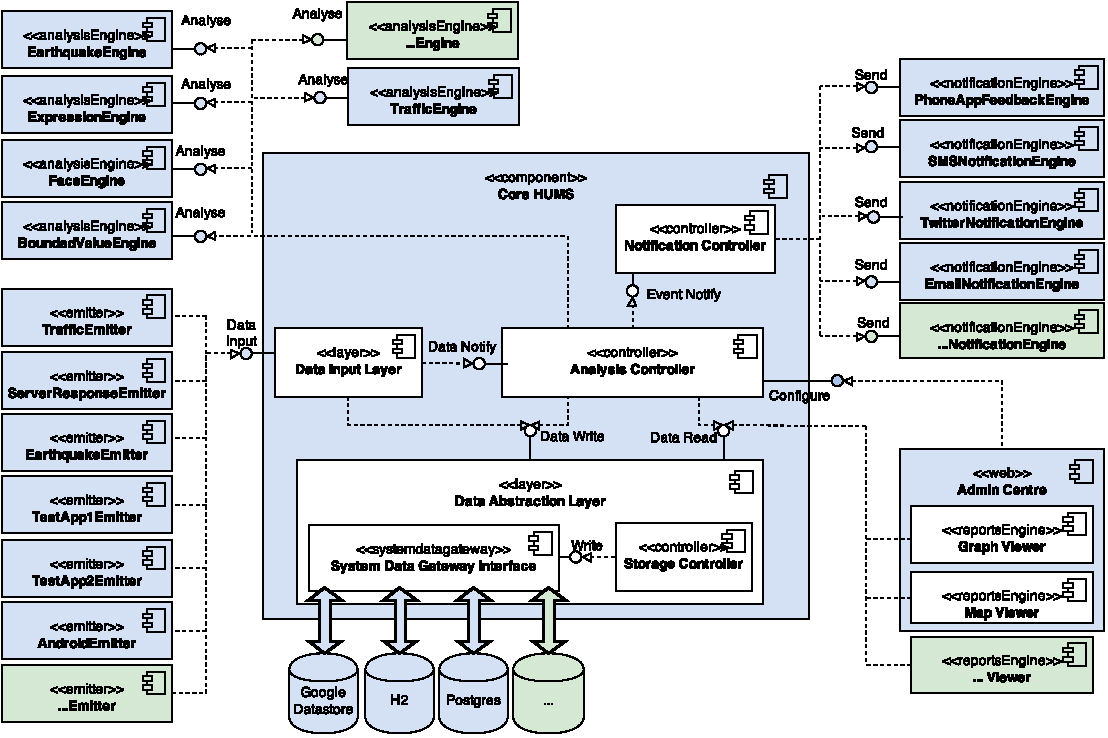
\includegraphics[width=\textwidth]{images/component.pdf}
  \caption{Module diagram of the System. The blue components and their contents have all been implemented. The green components are extensions left to the Consumer.}
  \label{fig:modules}
\end{figure}

\subsection{Component and Connector View}

In order to visualise how data flows through the system, from its inputs to its outputs, a \emph{Pipes and Filters} diagram of the HUMS has been created. This diagram, shown in Figure~\ref{fig:pipesAndFilter}, shows the distinct data transformation and processing filters in our solution, as well as the protocol of the pipes connecting them. Designing this diagram helped us to determine which pipes we must choose protocols for and which can be left for the client to define, improving the tailorability of the system by not unnecessarily restricting the Consumer.

The input to the HUMS, in this view, is the sensor data from the consumer system. This can be passed to the \texttt{:Emit Data} filter in any format, as this is the stage which converts client data to HUMS data. 

The \texttt{:Emit Data} filter transforms the client data into serialisable data which can be sent using protocol buffers to the \texttt{:Read Data} filter. Using \emph{Protocol Buffers}, allows for data to be sent locally or over a network, with or without encryption. 
The \texttt{:Read Data} filter de-serializes the client data and transforms it to a format which can be used with the Consumers defined datastore. 

The \texttt{:Store Data} filter inserts the data into the Consumers defined datastore.
The protocol of the pipes used to pass data to the \texttt{:Store Data} and the \texttt{:Create Report} filters are defined by the Consumer, being limited only by what their defined datastores support.
The \texttt{:Create Report} filter transforms data from the datastore into a \texttt{Data Report}, for example, a graph or PDF.

When sending data between the \texttt{:Store Data} and \texttt{:Analyse Data} filters, \texttt{SensorState} objects are passed, each of which hold the ID of a particular sensor, the timestamp of when it was created and stored, and its value at the time of creation. 

The \texttt{:Analyse Data} filter transforms \texttt{SensorState} objects into \texttt{Event} objects, which are used by the \texttt{:Generate Notification} filter to produce notifications using the engines specified by the client.
An \texttt{Event} object contains the ID of the system which caused the event, and a \texttt{Map} of key-value pairs containing information needed by the registered notification engines.

The \texttt{:Generate Notification} filter transforms an \texttt{Event} object into a notification, for example, an SMS or email. 

\begin{figure}[tbp]
  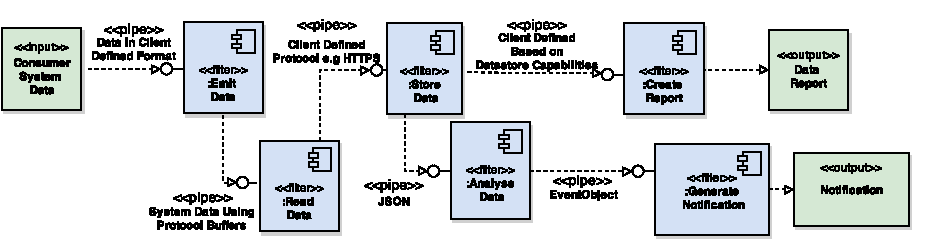
\includegraphics[width=\textwidth]{images/pipesAndFilters.pdf}
  \caption{A component and connector diagram of the HUMS, showing the protocols used when passing data between filters}
  \label{fig:pipesAndFilter}
\end{figure}

\subsection{Behavioural View}

A behavioural view can show the actual actions taken by the system when the data flows through the system, showing the different components and how they interact. Figure~\ref{fig:sequence} shows a sequence diagram that presents this information, detailing the different elements of the Core system and how it behaves during normal operation. Various methods and invocations are listed at the in the order that they occur, from top to bottom and left to right. The external parts of the system, such as the sources that data is gathered from and the destinations that notifications are sent to, are not shown.

\begin{figure}[tbp]
  \centering
  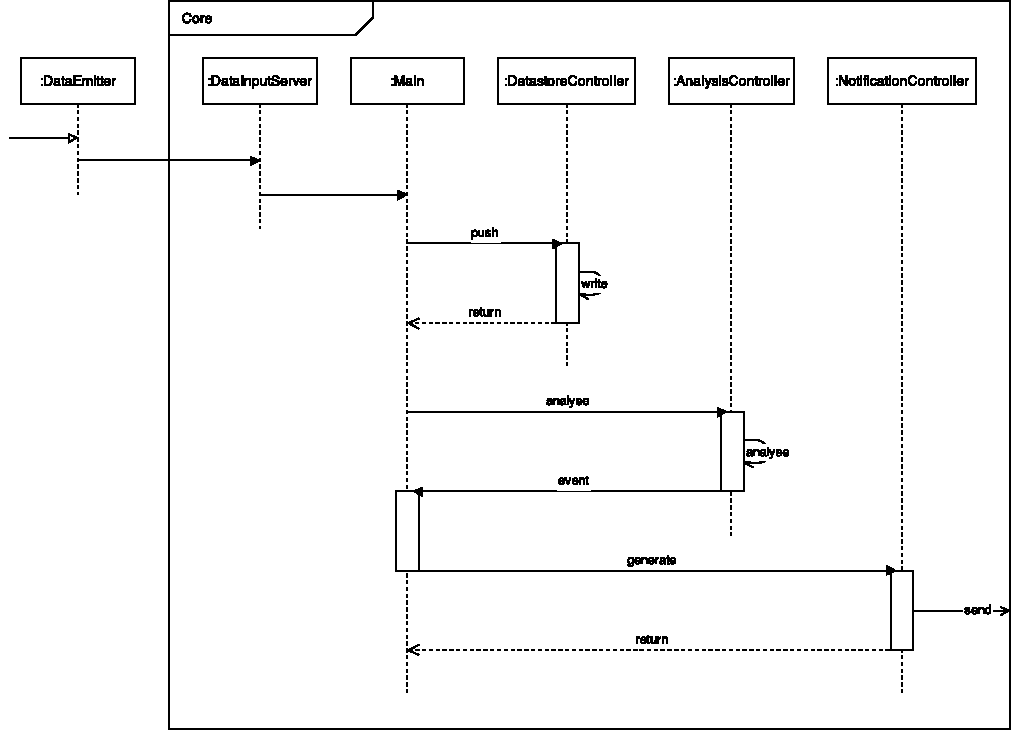
\includegraphics[width=\textwidth]{images/behaviourView.pdf}
  \caption{Sequence diagram showing the behaviour of the HUMS, using UML 2 notation}
  \label{fig:sequence}
\end{figure}


\subsection{Deployment View}
\hl{TODO Joe}
%-------------------------------------------------------------%
%-------------------DEVELOPMENT-------------------%
%-------------------------------------------------------------%
%   Notes: 					         	 %
%  	- Reference risks constantly, lots and lots	 %
%	- Reference requirements and scenarios 	 %
%-------------------------------------------------------------%
\section{Development}
\label{sec:dev}
\hl{TODO Prehaps Intro}

\subsection{Interim Implementation Summary}
\label{sec:interim_summary}
\hl{TODO ADAM}

\subsection{Changes Since the Interim Report}
\label{sec:changes}
\hl{TODO All}

\subsection{Core Development}
\label{sec:core}

The Core is the main application controlling the behaviour and functionality of the HUMS. It receives client data through Data Emitters and stores it using data storage engines, data is then passed to appropriate analysis engines, which can create \texttt{Event} objects that the Core passes on to the relevant notification engines.

\texttt{Controller} objects are used to dynamically load and manage the three different engine types. The use of dynamic class loading increases the configurability or modifiability of the system, by allowing the new engines to be added both at runtime and compile time. In addition, the Core automatically detects when new files are added to the folder they are loaded from, and refreshes the system. This means that from the Consumers perspective, they merely have to place their class into the correct folder, increasing the usability of the HUMS. 

Several example engines are provided with the HUMS and are described throughout this report. These engines implement standard interfaces provided with the HUMS Core, one for each of the three engine types: storage, analysis and notification. The Customer and Consumer can therefore easily extend and tailor the system by creating their own engines to meet their own needs.

The systems monitored by a particular HUMS instance, and how they will be monitored is defined using a \emph{JSON} configuration file.
The format of this file is displayed in Figure~\ref{fig:configFiles}, which shows the definition of a particular system, with a System ID, Sensor IDs, parameters, and which engines the system uses.
A configuration file is loaded into the Core by the Consumer before it is run. Changes to configuration files can be made manually through a text editor or in a more user-friendly manner through the Admin Centre.

\begin{figure}[tbp]
\begin{lstlisting}[language=json,firstnumber=1]
{
    "Systems": [
        {
            "SystemID": "EarthquakeMonitor",
            "Sensors": [
                {
                    "SensorID": "EQ",
                    "Params": {
                        "LOWER_BOUND": "1.0"
                    }
                }
            ],
            "Engines": [
                "EarthquakeAnalysisEngine",
                "TwitterNotificationEngine"
            ],
            "DatastoreGateway": "GWTSystemDataGateway",
            "Reporting": "Map"
        },
        etc...
    ]
}
\end{lstlisting}
\caption{An Example of the JSON configuration files used by the HUMS}
\label{fig:configFiles}
\end{figure}

Any changes made to the configuration file whilst the HUMS is running are automatically detected by the Core and cause the file to be reloaded allowing the alterations to take immediate effect. This reduces the Risk \emph{R.5} by ensuring the Consumer cannot forget to reload the file, increasing the usability of our HUMS by improving its learnability.

\hl{TODO Tom: Refactored to add config file that contains all it's parameters, which can be set and modified at runtime, separating params from the code}

In addition to the above, we created an optional GUI for our HUMS Core which makes the process of configuring and running our HUMS even simpler. Shown in Figure~\ref{fig:coreGUI}, this GUI allows the Consumer to select the configuration file they wish to use and to start and stop the Core with the click of a button. The GUI also keeps the Consumer informed of what the Core is doing through an integrated console, which reports any errors such as incorrectly formatted configuration files, as well as the general status of the Core. The GUI was created using the \emph{Standard Widget Toolkit} \cite{swt}, this was chosen over other UI libraries, such as \emph{Swing}, as it uses native components, increasing user efficiency and satisfaction by using components they are already familiar with.

\begin{figure}[tb]
\centering
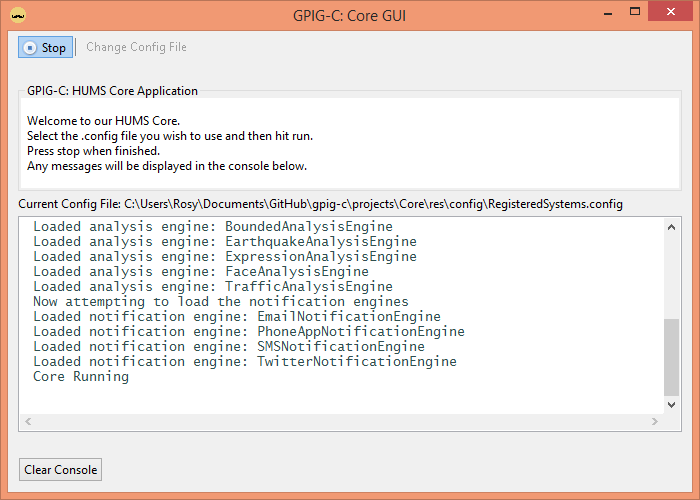
\includegraphics[width = \textwidth]{images/coreGUI.png}
\caption{A Screenshot of the Core GUI}
\label{fig:coreGUI}
\end{figure}
A lightweight Jetty server was also added to the Core demonstrating that the Admin Centre can be served from the same system that the Core runs on. This enables further integration between the configuration files and the web interface created for easily administering them, and avoids any custom server having to be manually set up by the Consumer by automating the process. The functionality of the Admin Centre is described further in Section~\ref{sec:admin}. 

\subsection{Project Management}
\hl{TODO Joe}

\subsection{Sensing}
\label{sec:monitor}
In this section we describe what data our HUMS currently monitors. We created six sample Data Emitters for this stage of the project, in order to demonstrate the tailorability of our HUMS. These show how the HUMS can integrate with existing applications, and APIs, as well as how it can be used with specially made applications. An Consumer would be able to quickly create a Data Emitter for their own application by using the interfaces provided with our HUMS.

\subsubsection{Test Applications} \label{subsec:tapp}
Part of our task was monitoring the provided test applications, treating them as black-box systems we knew nothing about. For the first we simply monitored the memory and CPU usage, but for the second we also added state, number of threads, last processor it was run on, and working directory. For this we created a process monitoring engine which is capable of tracking information from a process.

The monitoring engine utilises the System Information GAthereR (SIGAR) API. SIGAR is a cross-platform API which allows system information and process information to be read, without worrying about which implementation for reading that information the platform provides. The information gathered by this engine is forwarded to the core for analysis.

\subsubsection{Earthquakes and Traffic}
In order to ensure our HUMS is capable of receiving, analysing, and reporting data through various external APIs, we updated our earthquake Data Emitter and added an additional traffic Data Emitter, monitoring real time UK traffic accidents and incidents. The earthquake data (from the U.S. Geological Survey~\cite{us_geo}) is in a JSON format and the traffic data (from the UK Highways Agency~\cite{ha_traffic}) is in an XML format, which are both standard and commonly used data formats. These two emitters demonstrate the extensiblility of the HUMS as similar additional Data Emitters can easily be created to read data from other sources, which would likely also use XML or JSON formats.

\subsubsection{Server Responsiveness}
A common use of existing HUMS systems is in monitoring the responsiveness of websites and servers, alerting users and staff if the system becomes unavailable. In order to ensure our HUMS was capable of such a task, we implemented a response time data emitter which determines the response time of requests to a given website\footnote{thalesgroup.com} and sends this data to the core for analysis.

\subsubsection{Emitter Launcher}
The demonstration purposes, and to make our prototype easier to test and use, we created an \emph{Emitter Launcher}, which simplifies the process of running our desktop Data Emitters by allowing the individually packaged emitters to all be run from a single application, using a GUI. A screenshot of this GUI is shown in Figure~\ref{fig:launcherGUI}, it has again been created using the \emph{Standard Widget Toolkit} \cite{swt}, meaning native components can be used.
 
\begin{figure}[tbp]
\centering
\includegraphics*[width=0.8\textwidth]{images/launcherGUI.png}
\caption{A screenshot of the Emitter Launcher GUI}
\label{fig:launcherGUI}
\end{figure}

\subsubsection{Android Mobile Application}
\hl{Tom}
To explore the possibilities surrounding monitoring remote systems over network communication, we created an Android application, with three test systems allowing us to demonstrate that our HUMS is capable of this. Screenshots of the Android application are shown in Figure~\ref{fig:android}.

The first system simulates a car monitoring system, allowing users to select values for a number of sensors and then push them to the remotely-based core. In the real system, the user would not set the values or manually push them---it would all be automatic---however, we choose to manually update the data for the purposes of demonstrating the functionality.

The second system is a phone battery monitoring system, which allows the user to define how long they would like to use their mobile device for and based on the given battery life, uses the HUMS to determine which services can stay on in order for this target to be met. The HUMS feeds back into the phone system, toggling services as necessary to balance device functionality and battery usage. This system was designed to show how our HUMS is capable of monitoring a system, and feeding information back to alter the systems behaviour in response to the information it collects.

The final system performs face recognition, collecting face data using the built-in camera, forwarding that data to the HUMS for analysis and, if appropriate, notification. This system was included to show how our HUMS allows for fast, complex, and specific data analysis, in this case using computer vision algorithms, in order to show that risk \emph{R.8} has not been realised. Section~\ref{sec:fae} describes the details of our computer vision approach.

\begin{figure}[tbp]
\centering
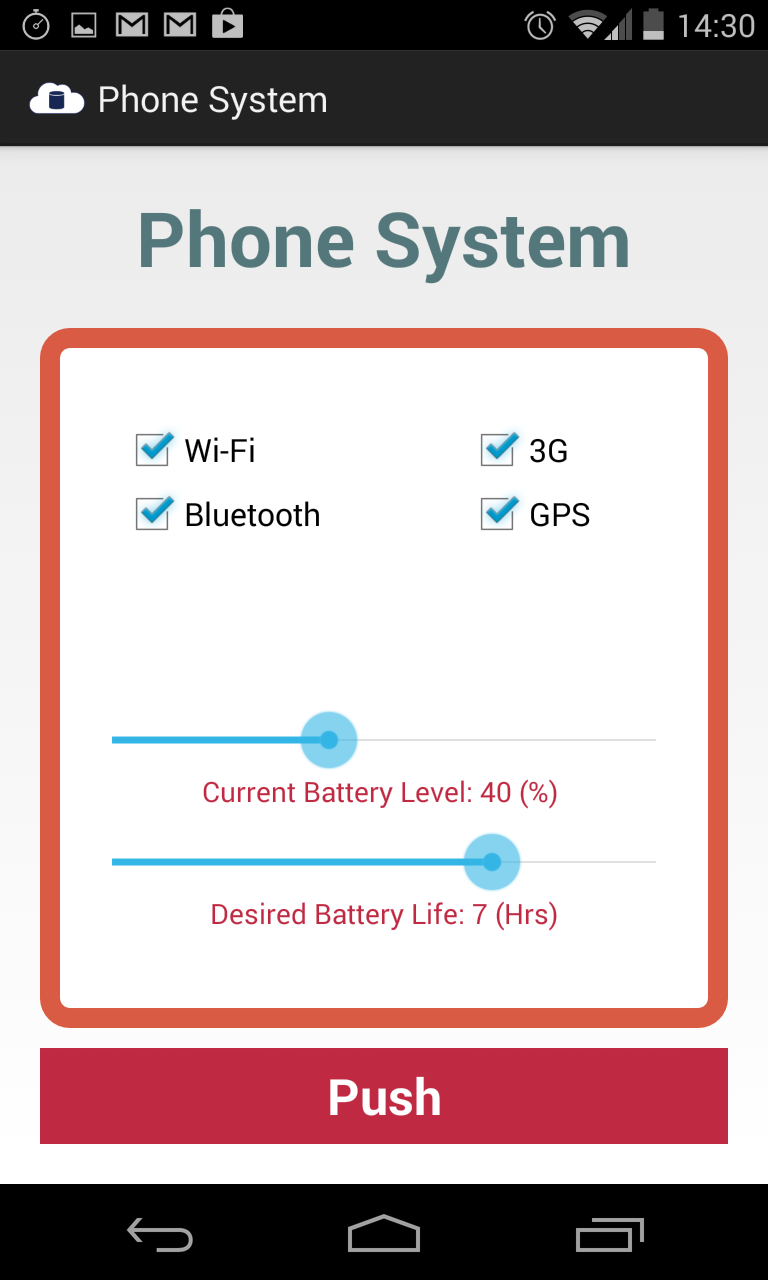
\includegraphics[width=4.3cm]{images/phoneApp.png}
\hspace{0.5cm}
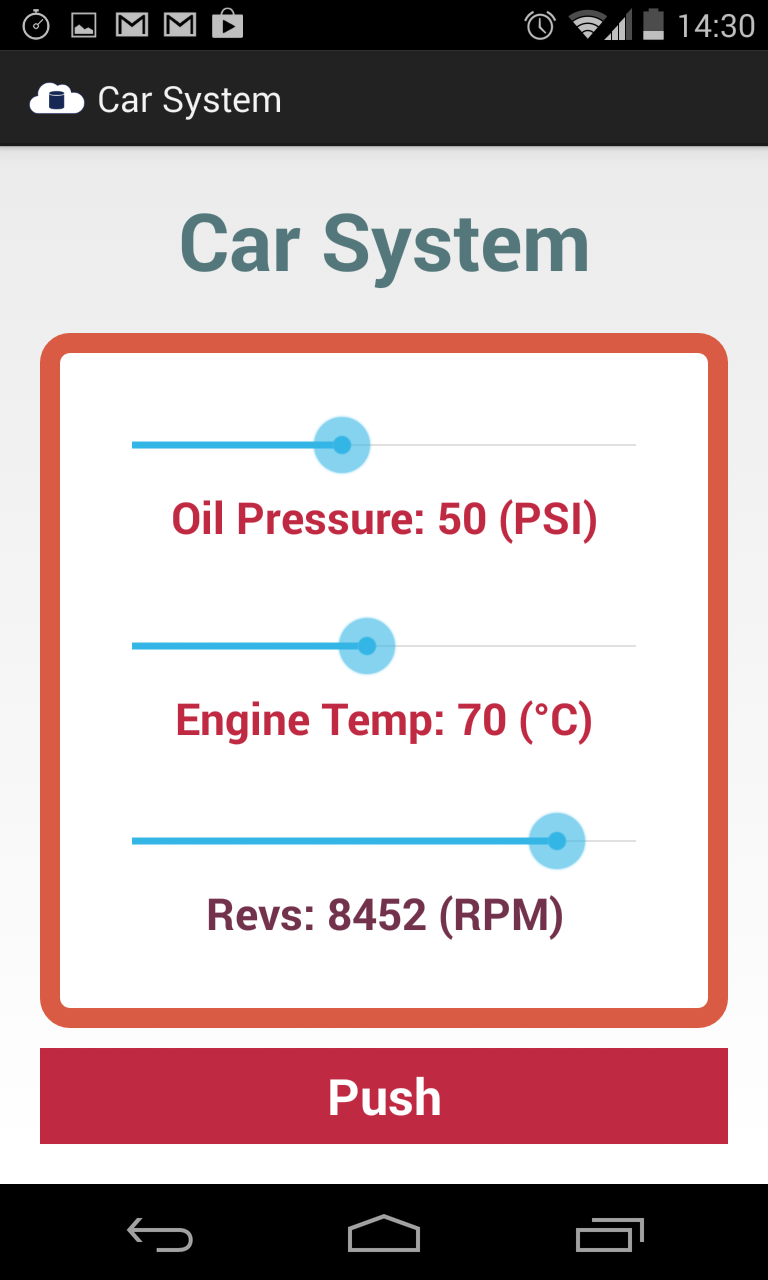
\includegraphics[width=4.3cm]{images/carApp.png}
\hspace{0.5cm}
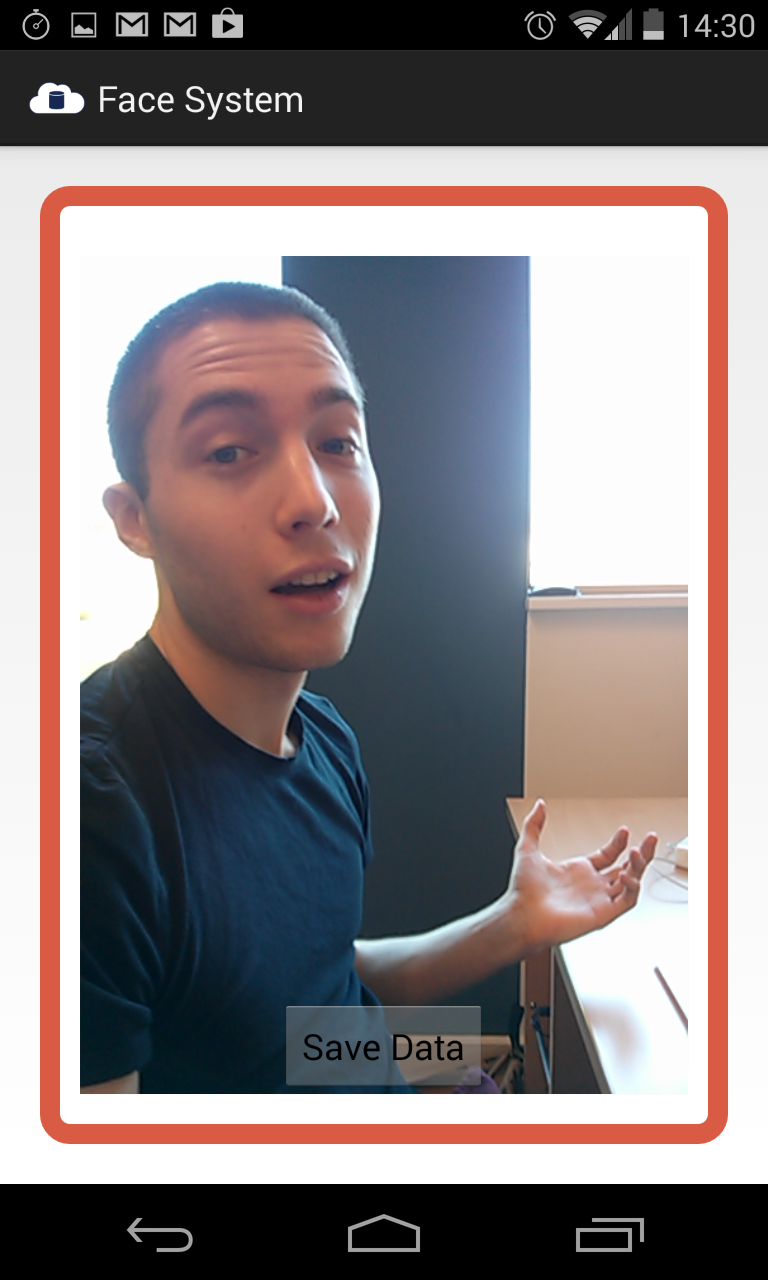
\includegraphics[width=4.3cm]{images/faceApp.png}
\caption{Screenshots of the Android mobile application, showing each of the three subsystems.}
\label{fig:android}
\end{figure}


\subsection{Storing}
\label{sec:store}
This section describes how our HUMS implementation stores data. Our HUMS provides a generic \texttt{SystemDataGateway} interface which can be implemented for a variety of existing datastores. To demonstrate this we created \hl{how many} sample implementations interfacing with a variety of popular storage solutions, including: \emph{Google App Engine}, \emph{PostgreSQL}, \hl{XXX}, and \emph{H2}. This was done to show how our system does not force the Consumer to conform to a particular data schema or datastore, in fact, the datastores registered to our sample systems can be altered in the configuration file without any errors occurring. This method increases the overall tailorability of our solution whilst addressing risks \emph{R.7} and \emph{R.8}. The remote datastores used in our implementation were chosen as they allow \emph{NFR.9} be achieved.

Prepared statements were used where possible in our datastore implementations, being compiled once and then reused, leading to significant gains in performance. Prepared statements also offer improved security against SQL injection attacks, with all user input being treated as data and thus not altering the characteristics of data queries.

\subsubsection{Google App Engine Storage}
\emph{Google App Engine} is a popular cloud based Platform as a Service (PaaS) solution, which is used to deploy applications and manage data. We choose to use this as part of our implementation to demonstrate how our HUMS can easily interface with a remote, NoSQL, datastore. We did this by creating and hosting a simple web-based application on \emph{Google App Engine}, and then communicating with it using a \texttt{SystemDataGateway} object which performed the relevant HTTP requests.  

\subsubsection{PostgreSQL Storage}
\emph{PostgreSQL} is a prominent relational database management system, which is queried using SQL and is ACID compliment. We included this storage engine in order to show how our HUMS can interact with a remote SQL datastore. 
To implement this we created an \emph{Heroku} web application, which included a \emph{PostgreSQL} database, and communicated with it from a \texttt{SystemDataGateway} object, again using HTTP.

\hl{For this implementation we were able to use a connection pool, which provides a cache of reusable database connections. This means that connections only need to be created once and shared between components that require data access. The HikariCP Java library was used to simplify the implementation of database connection pools. ---- REMOVE?}

\subsubsection{H2 Storage}
For real-time applications that require high performance and low response times a local H2 instance is offered. H2 is a Java library that implements a simple, self-contained and server-less, transactional SQL database. H2 can be run in embedded or server mode, its small storage footprint of $1.5$MB and low memory usage make it ideal for use in resource constrained environments. 


\subsection{Analysing}
\label{sec:analysis}
In this section we describe how our HUMS implementation currently analyses data. We created five sample analysis engines for this stage of the project, demonstrating the flexibility of our HUMS, performing both complex and simple analysis. These engines show how the HUMS can be used for a variety of analysis applications, and how easy it is for the Consumer to add additional engines using the generic \texttt{AnalysisEngine} abstract class provided.

\subsubsection{Generic Bounded Sensor Value Engine}

The previous mean analysis engine has been rewritten to form a generic bounded sensor value engine. This engine performs analysis on each sensor in the system being analysed to determine if the mean average of the values is outside of specified bounds. It then produces a single event detailing any violations across all the sensors, which generates a single notification for the system being analysed rather than a flood of them.

The number of data records to average over and the upper and lower bounds for the acceptable range of the average are specified for each sensor in the configuration file. This allows these parameters to easily be changed by the User to tailor to their needs, and also adds configurability on a per sensor level.

The average computed is a moving average over a certain number (depending on the value specified in the configuration) of the last records in the database. The engine is able to do this across any sensor that records numerical values so is reusable across different contexts and flexible to different uses of the HUMS.

\subsubsection{Generic Expression Engine}
\hl{TODO Tom}
We devised a generic expression engine, \texttt{ExpressionAnalysisEngine}, which allows the configuration file to describe a wide range of potential analysis processes, avoiding the need to build new analysis engine classes. The expression engine supports most reasonable closed-form expressions, as well as less common, but helpful features such as conditional expressions. Figure~\ref{fig:exprExample} gives an example of an expression that can be given in the system configuration file to define the action of the engine.
\begin{figure}[htbp]
\centering
\verb+if(max(ENGINE_TEMP_A, ENGINE_TEMP_B) >= 120 or RPM > 5000, -1, 0)+
\caption{A basic example of an expression that evaluates to $-1$ when a system is operating outside of its defined normal operational parameters.}
\label{fig:exprExample}
\end{figure}

The values of variables which represent the state of the system being monitored are available in the expression, and are evaluated lazily for efficiency (evaluation often entails querying the datastore to retrieve the most recent value, potentially over a network connection, which could be very inefficient when unnecessary).

Since the expressions that may be passed to the \texttt{ExpressionAnalysisEngine} can be arbitrarily large, a limit may be imposed on the processing time that may be taken to evaluate an expression. If that time limit is broken, the engine stops processing the expression and sends a notification to the appropriate users to warn them of the situation.

The implementation of the \texttt{ExpressionAnalysisEngine} works towards addressing the tailorability quality attribute of the solution, particularly its flexibility and configurability, allowing the HUMS to be easily customised by the Consumer without needing any particular software engineering knowledge. % TODO Expand on this?

% TODO The library used?

\subsubsection{Face Analysis Engine}
\label{sec:fae}

\hl{TODO Tom/Joe Face Recognition for Security}
% TODO Separate analysis from sensing
The Android app collects face data, forwarding it to the Core for analysis, where notifications are generated, notionally granting or denying access to a secure system. This module shows off the ability of sensors and analysis engines to work together to perform complex tasks, which can be tailored using the Core configuration file.

The face recognition process is two fold: An image is captured and its dimensionality is reduced by the Android app before being sent on to the Core, then the \texttt{FaceAnalysisEngine} takes this face description and analyses it to decide if the face is authorised or not.

The face description in the Android app is computed using the Local Binary Patterns Histogram (LBPH) \cite{ahonen2006face} method. Each pixel in the image is reduced to a bit-vector describing whether each of the neighbouring pixels is brighter or darker than it (although what constitutes a neighbour can be varied to control for scaling). These bit-vectors are then used to generate a histogram. All \emph{uniform bit patterns}, those which have at least two $1$s in a row and no more than two transitions between runs of $1$s and $0$s, have a separate bin and all other patterns have a single bin. A histogram is made for each of a fixed number of regions in the image to ensure that some degree of locality is kept. Each histogram is then concatenated to create the full description vector---the \emph{spatially enhanced histogram}. This results in a compressed description of the image which attempts to preserve the information content pertaining to face description. This is the data which is then transmitted to the Core.

When the histogram data is received by the \texttt{FaceAnalysisEngine}, it is compared against the example authorised faces using the Chi-Squared distance measure, authorising the face provided by the sensor if its distance from any of the example authorised faces provided by the configuration file is less than some threshold, also given by the configuration file, and any example unauthorised face.

% TODO This method is robust to lighting and pose \cite{ahonen2006face} (due to use of local thresholds)

\subsubsection{Other Analysis Engines}
The \texttt{TrafficAnalysisEngine}, creates an event when a reading is generated, the analysis performed in this case is simply parsing the data about the earthquake and putting it into a readable format for the registered notification engine. The \texttt{EarthquakeAnalysisEngine} is similar, parsing CSV data about an earthquake and then creating a notification \texttt{Event} only if the magnitude above a specified value, so larger earthquakes generate events. These engines show how simple the analysis components can be, going to prove that the \texttt{AnalysisEngine} abstract class in incredibly versatile  Other analysis engines, the analysis system can be easily built up. Hence, it is easy to add further analysis engines to the system. This can easily be done by extending the \texttt{AnalysisEngine} abstract class, and implementing the required methods.


\subsection{Reporting and Notifying}
\label{sec:reporting}

This section describes the reporting and notification capabilities of our HUMS. Events created by analysis are used to create notifications using any notification engines configured for a particular HUMS instance. We created four example notification engines to demonstrate a range of different types of notification that might want to be generated and dispatched by a HUMS, and to show the flexibility and tailorability of the system. They exhibit how the Customer or Consumer could easily create custom notification engines by implementing the generic \texttt{NotificationEngine} abstract class provided, and can easily choose which engines to use for different systems using the configuration file.

For reporting, two sample reporting engines were created that can be used through the Admin Centre. Once requested by the User, these generate reports with live updating information from the HUMS. These engines provide just a small idea of what is possible with our HUMS implementation, with further web based or standalone reporting engines -- or engines integrated into other applications -- able to be created to interact with the system and produce other types of reports the User may require.

\subsubsection{SMS Notifications}
A notification engine was created than can send SMS text messages to mobile phones. This is useful functionality for a HUMS due to the near ubiquitousness of mobile phones in modern life; a User is likely to have their phone with them most of the time so can instantly be notified and informed of anything the HUMS needs to flag up, and then react appropriately. It is a quick and efficient notification method and one that works across all phone platforms. To build this engine we utilised the service offered by the communications company Twilio~\cite{twilio}, who have a large infrastructure for telecommunications and offer an easy to use API.

\subsubsection{Email Notifications}
The \texttt{EmailNotificationEngine} provided has the same functionality as the engine included in the interim report, however, has been heavily re-factored to comply with our new, more modular code-base.
It can be configured to send email notifications for events to any email address, and may be useful for more detailed, less frequent notifications. This has been implemented using the Apache Commons Email~\cite{ac_email} library for Java to interact with an email account over IMAP and SMTP.

\subsubsection{Twitter Notifications}
The \texttt{TwitterNotificationEngine} provided allows events to be pushed to the social networking site \emph{Twitter}. We included this engine to demonstrate how our HUMS implementation can be used to interact with popular platforms to provide report events, such as earthquakes and traffic information, to the masses. The engine creates a tweet from the message it receives from analysis engines and then pushes that tweet to the registered account. This has been implemented using the Twitter4J~\cite{twitter4j} Java library to access the Twitter API.

\subsubsection{Android Application Feedback Notifications}
\hl{TODO Rosy}

\subsubsection{Map Report}
The map reporting engine created in the interim report was improved on, making it into a more generic reporting engine that can be used with any latitude and longitude data. This is demonstrated through its use with both the earthquake and the traffic data. Map reports are generated on demand by the User through the Admin Centre, and can then automatically update with the latest data that is input to the HUMS to provide live information. The map generated uses the Google Maps JavaScript API~\cite{g_maps} which is customised to fit the needs of the report.

\subsubsection{Graph Report}
Similarly to the map reporting engine, the graph reporting engine has been enhanced since the interim report and is now a separate engine that can be used to graph different data. The data from both test applications is graphed in the Admin Centre using this engine, showing its configurability of use. The graph reports generated can also automatically update to show live data. This report uses the open source Chart.js JavaScript charting library~\cite{chart_js} to draw and customise the graph.

\subsection{Admin Centre}
\label{sec:admin}

The prototype Admin Centre previously created has been updated and refined to provide a central locations for the User to control the operation and settings of the HUMS. By offering this through a web interface it provides a more familiar and user friendly way for the configuration to be viewed and edited without having to manually edit configuration files. It also means that the Admin Centre can be accessed remotely from a number of different devices and not just from where the core is being run.

The Admin Centre also provides the reporting facilities of the HUMS, with two example reporting engines currently created. A graph report is available and can be used with data like that from the first and second test applications, and a map report is available which is more applicable to data from the earthquake or traffic monitoring.

The updates to the Admin Centre have developed the previous prototype into a fully functioning system that integrates with the HUMS and presents real data and options to the User that they can interact with and update to have effect on the running HUMS instance.

\begin{figure}[h!b]
    \begin{subfigure}{0.49\textwidth}
        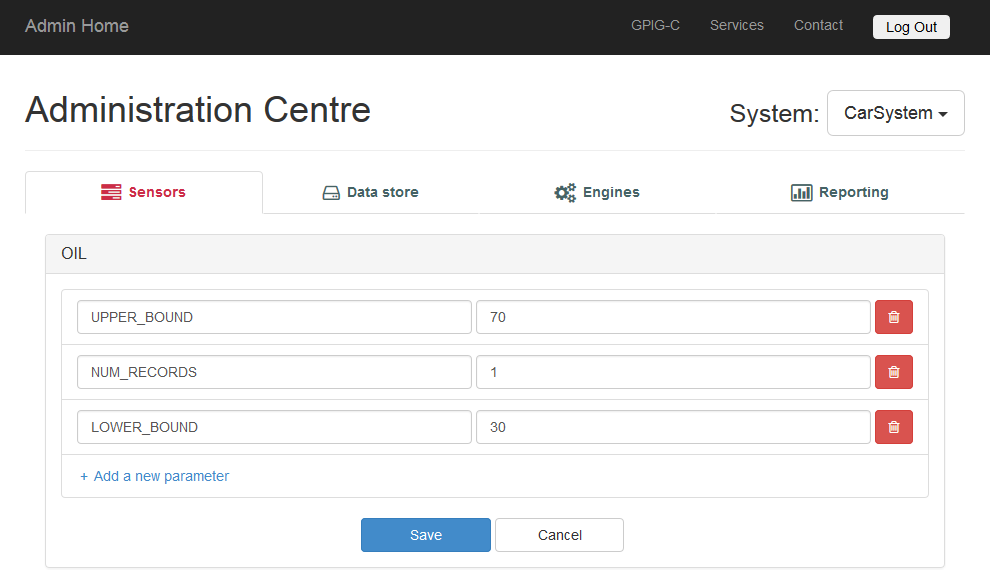
\includegraphics[width=\textwidth]{images/admin-centre_sensors.png}
        \caption{Sensors}
        \label{fig:admin-centre_sensors}
    \end{subfigure}
    ~
    \begin{subfigure}{0.49\textwidth}
        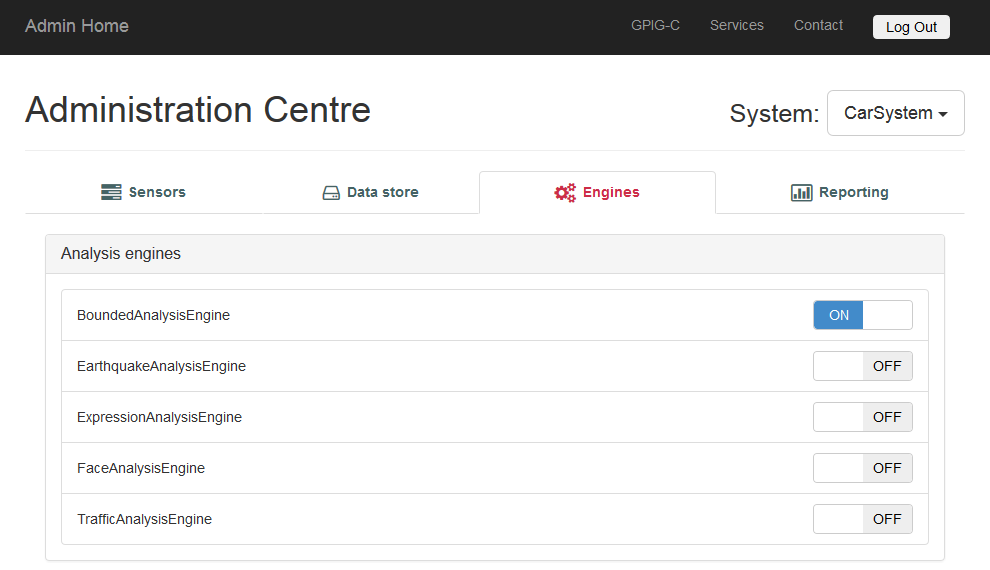
\includegraphics[width=\textwidth]{images/admin-centre_engines.png}
        \caption{Engine}
        \label{fig:admin-centre_engines}
    \end{subfigure}
	\vspace{0.2cm}

    \begin{subfigure}{0.49\textwidth}
        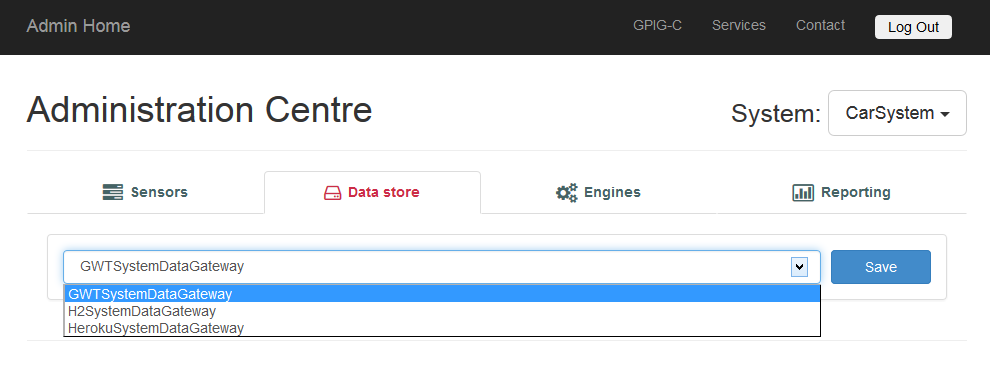
\includegraphics[width=\textwidth]{images/admin-centre_data.png}
        \caption{Data store}
        \label{fig:admin-centre_data}
    \end{subfigure}
	~
	\begin{subfigure}{0.49\textwidth}
        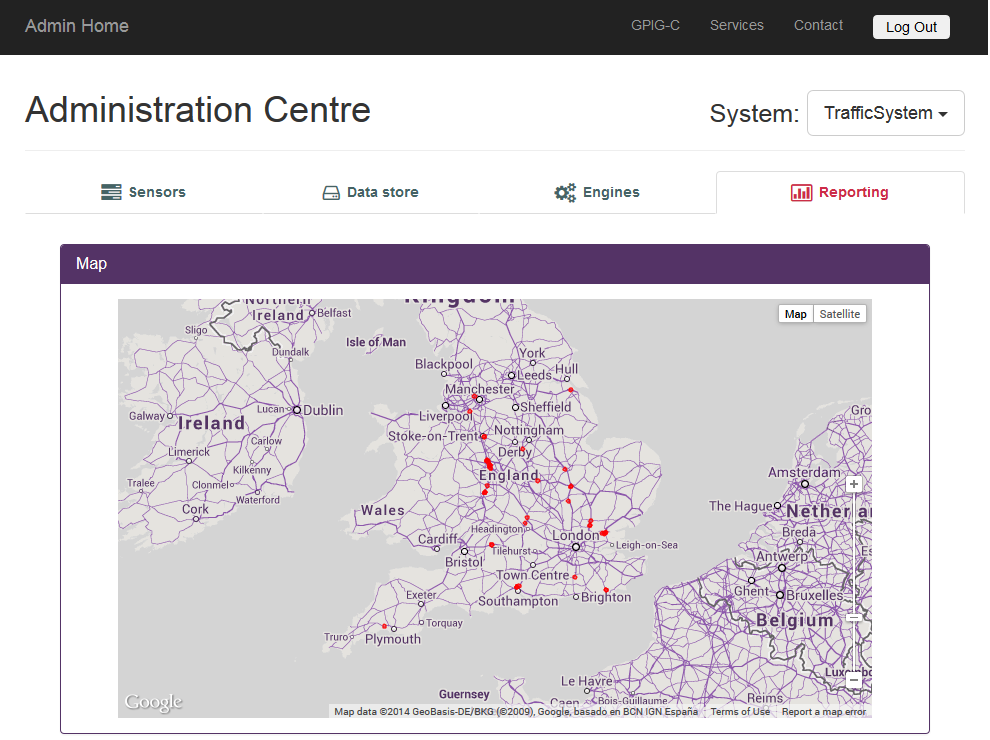
\includegraphics[width=\textwidth]{images/admin-centre_report.png}
        \caption{Reporting}
        \label{fig:admin-centre_report}
    \end{subfigure}
    \caption{Screenshots of the Admin Centre}
	\label{fig:admin-centre}
\end{figure}

%-------------------------------------------------------------%
%-----------------------TESTING-----------------------%
%-------------------------------------------------------------%
\section{Testing}
\label{sec:testing}

\hl{TODO!}


%-------------------------------------------------------------%
%-----------------------PROTOTYPE-----------------------%
%-------------------------------------------------------------%
\section{Prototype Implementation Evaluation}
\label{sec:prototype}
\hl{INTRO: Rosy||Joe||Andy}

\subsection{Evaluation Against Requirements, Qualities, and Scenarios}
\label{sec:req_eval}
\hl{TODO Ant}
% -- Qual attibrs
% High configurability
% High modifiability
% High Interop
% High Avail
% High Security
% Medi Performance
% Medi Testability
%  Low Usability

% -- scenario qual atr
% QAS1 The Customer wishes to reconfigure the system to monitor mechanical systems.
% QAS2 The Customer wishes to add an additional analysis, reporting, or notification engine to the HUMS.
% QAS3 The Client is authenticated, and allowed to access system services, or is not recognised and blocked from accessing system data and services.
% QAS4 A Notification is sent to the administrator of the HUMS instance, and the HUMS periodically attempts to reconnect to the Datastore


To consider the meeting of requirements, we lay out here the steps which we have taken in order to validate the meeting of the requirements.

\tableformat{| l | l | l |}{ \hline	FR.x  & 	Description of FR  & 	What we did \\ \hline
	FR.1  & 	  & 	We created an API for data input which uses a system ID to determine which input is sending the data. The information is sent to the core utilising a data emitter and this data emitter can read the sensor ID and pass the information into the analysis engine for analysis. \\ \hline
	FR.2  & 	  & 	Timestamps are held for all data, and stored in the data store when the information is saved. \\ \hline
	FR.3  & 	  & 	To meet the requirement to store correctly structured data, we have enforced checks on data entering the core. The data is stored in a database. This is H2 for a local database, and is a postgres instance on heroku for the cloud solution. \\ \hline
	FR.4  & 	  & 	This requirement has been satisfied by the use of configuration files, these can be loaded into the core at runtime. And can easily be changed and reloaded while the core is running. The administration center can be used to edit these configuration files even while the system is running. \\ \hline
	FR.5  & 	  & 	The requirement for notifications on a full quota were meant for the SaaS part of our implementation. As this is a prototype and is not completed, this is not currently implementation. \hl{?} \\ \hline
	FR.6  & 	  & 	  \hl{?} \\ \hline
	FR.7  & 	  & 	  \hl{?} \\ \hline
	FR.8  & 	  & 	 \\ \hline
	FR.9  & 	  & 	For recognition of an event, the information which is received from a system ID is passed into the core and analysed. If analysis rules are matched, then a notification is generated for the event. \\ \hline
	FR.10  & 	  & 	 \\ \hline
	FR.11  & 	  & 	 \\ \hline
	FR.12  & 	  & 	This can be achieved by the user placing them in the correct namespace in JAVA. The system will load all the classes associated with the engines when it first loads. \\ \hline
}{Evaluation for Satisfaction of Functional Requirements}{frevaltable}

\tableformat{| l | l | l |}{ \hline	NFR.x  & 	Description of NFR  & 	What we did \\ \hline
	NFR.1  & 	  & 	The data store is not within the HUMS hardware, but is instead user defined. Hence, the system is capable of keeping data persistently even when the hardware the HUMS is operated on is changed. \\ \hline
	NFR.2  & 	  & 	There has been a README provided. \\ \hline
	NFR.3  & 	  & 	The HUMS system can be utilised regardless of geographic location, as the main monitoring site is accessible from the web. Furthermore, the emitters can be run detached from the main system, for example on an embedded system. \\ \hline
	NFR.4  & 	  & 	\hl{We didnt implement security} \\ \hline
	NFR.5  & 	  & 	\hl{!} \\ \hline
	NFR.6  & 	  & 	The tests for the system have been created and included at each stage of the development. \hl{write smat stuff} \\ \hline
	NFR.7  & 	  & 	The system has not currently been performend. However, in the case of the real system, this would be performed by the customer and the customer would sign off to show the requirements were met. \\ \hline
	NFR.8  & 	  & 	The current implementation is executing with 5 clients. With the emitter launcher we have tested it with 5 clients and the performance is correct. There have been tests with more clients and the functionality remains correct. \\ \hline
	NFR.9  & 	  & 	The heroku instance has an uptime which satisfies this requirement. \\ \hline
	NFR.10  & 	  & 	\hl{data backup - adam?} \\ \hline
	NFR.11  & 	  & 	 \\ \hline
	NFR.12  & 	  & 	 \\ \hline
	NFR.13  & 	  & 	To achieve this, a key-value data store format has been used. This relaxes the need for a schema to a simple pair of key to value. \\ \hline
	NFR.14  & 	  & 	The format for the configuration files is JSON, this is a widely-adopted nad easy to modify format for update by a human. \\ \hline
}{Evaluation for Satisfaction of Non-Functional Requirements}{nfrevaltable}


The quality attributes laid out in Section~\ref{sec:scenarios} have been largely satisfied. The requirement that the HUMS system be utilisable in multiple domains was emphasised strongly, and so high configurability was a goal from the beginning of the project. One are important to the customer was the ability to monitor mechanical systems. This can be achieved using our HUMS system, and a stand-alone data store to log the information. This would work in a similar manor to a black box recorder, and the data could be easily retrieved when needed. The notification system could easily be adapted to turn, for example, an LED off/on when an error had occurred.

A scenario for evaluating the modifiability is the ability to add engines for analysis, reporting or notifications. This has been achieved using extensible APIs for the analysis, reporting and notification engines. Each of the engines contains an abstract base class which can be extended to provide a new engine. For example, to implement a new analysis engine one must simply extend the AnalysisEngine class and implement the required abstract methods.

To evaluate the security, we created a scenario whereby a unknown client would attempt to access data stored in the HUMS or would attempt to insert data into the HUMS. Whilst we have not implemented the security system in the deliverable, we have theorised about how we would go about it and if we had more time in order to implement the full system, we have stated how we would achieve a given level of security.

\subsection{Evaluation on Test Application 1}
\label{sec:test_app1}

We decided to monitor the memory and CPU usage of the test application, and our initial implementation simply queried the operating system for these values, using the SIGAR library. However, this did not work as the JVM manages its own heap internally. We then changed to directly querying the target JVM for its memory usage using the JMX libraries, which was successful.

By using these cross-platform and established libraries, our monitor can be generalised to more than just the test application. This is illustrated by how easily we were able to reuse it as the basis of the second test application.

\subsection{Evaluation on Test Application 2}
\label{sec:test_app2}

Using iotop under Ubuntu 14.04, we were able to verify that the test application did not perform any notable IO operations. Using Wireshark under the same system, no network activity was detected either.
We decided to monitor the process memory usage, CPU usage, state (idle, running, sleeping, stopped, or zombie), working directory, number of threads, and which processor it was last run on. We were able to base the monitor on that developed for the first test application with only minor changes. We decided to monitor the threads because none of the other metrics produced an interesting result, however we found that only one thread was used.

\subsection{Evaluation of the HUMS SaaS}
\label{sec:hums_saas}
\hl{TODO Andy}
% also mention PaaS here?


\subsection{Evaluation of Additional Engines}
\label{sec:additional}
\hl{TODO Rosy\&Tom\&Adam}


\subsection{Instructions for Running and Replicating Results}
\label{sec:instructions}
\hl{TODO! - super easy GUIs, sources online, etc}


%-------------------------------------------------------------%
%---------------------COMMUNICATION-------------------%
%-------------------------------------------------------------%
\section{Customer Communication}
\label{sec:customer_comms}

We maintained communication with the Customer throughout the phase of this report, with emails exchanged every few weeks. The first feedback received from the Customer was the feedback to the previous Interim Report. This was in the form of written feedback and a face-to-face meeting with the Customer, with the main points raised for improvement surrounding the risks and the quality attribute scenarios. This feedback was taken on board and incorporated into this report, with risks more thoroughly considered throughout the process and with the scenarios explicitly defined.

During email communication with the Customer, we attempted to resolve an issue they had with accessing the web sources that were produced as part of the Interim Report. Once this was done we briefly discussed the ideas behind the configurable engines architecture and it was agreed that it was a good strategy. We then asked about different qualities expected of the system, particularly configurability and its related qualities. The Customer replied highlighting configurability as a key quality and this helped to influence some of our development to ensure that this was well met.

Further information about how development was progressing and the proposals for future work was exchanged to keep the Customer up-to-date and ensure that it was on the right track. This included information about how the system would meet the previously highlighted configurability quality, and how this could be achieved at compile time and run time.


%-------------------------------------------------------------%
%----------------------CONCLUSION----------------------%
%-------------------------------------------------------------%
\section{Conclusion}
\label{sec:conclusion}
\hl{TODO All}

\subsection{Summary}
\label{sec:summary}
\hl{TODO All}

\subsection{Reflection}
\label{sec:reflection}
\hl{TODO All}

\bibliography{report-refs}
\bibliographystyle{IEEEtran}
\end{document}

